\documentclass[border=4pt]{standalone}
\usepackage{tikz}
\usetikzlibrary{arrows.meta, calc, positioning, fit, backgrounds}
\usepackage{amsmath, amssymb}

% Palette shared with fig_interleaved_pipeline.tex
\definecolor{gnnblue}{RGB}{70,130,190}
\definecolor{gnnfill}{RGB}{210,228,248}
\definecolor{bpgreen}{RGB}{60,155,90}
\definecolor{bpfill}{RGB}{210,240,215}
\definecolor{filmorange}{RGB}{210,120,40}
\definecolor{fillfill}{RGB}{252,235,205}
\definecolor{iogray}{RGB}{100,100,100}
\definecolor{iofill}{RGB}{235,235,235}

% Matches gnn_pipeline/gnn_model.py (TannerGNN, TypedMessagePassingLayer):
% input projection Linear->LayerNorm->ReLU; per edge type an MLP on [h_src||h_dst];
% sum aggregation; optional FiLM on the aggregate; GRU update; residual; LayerNorm;
% readout MLP on variable nodes only.

\begin{document}
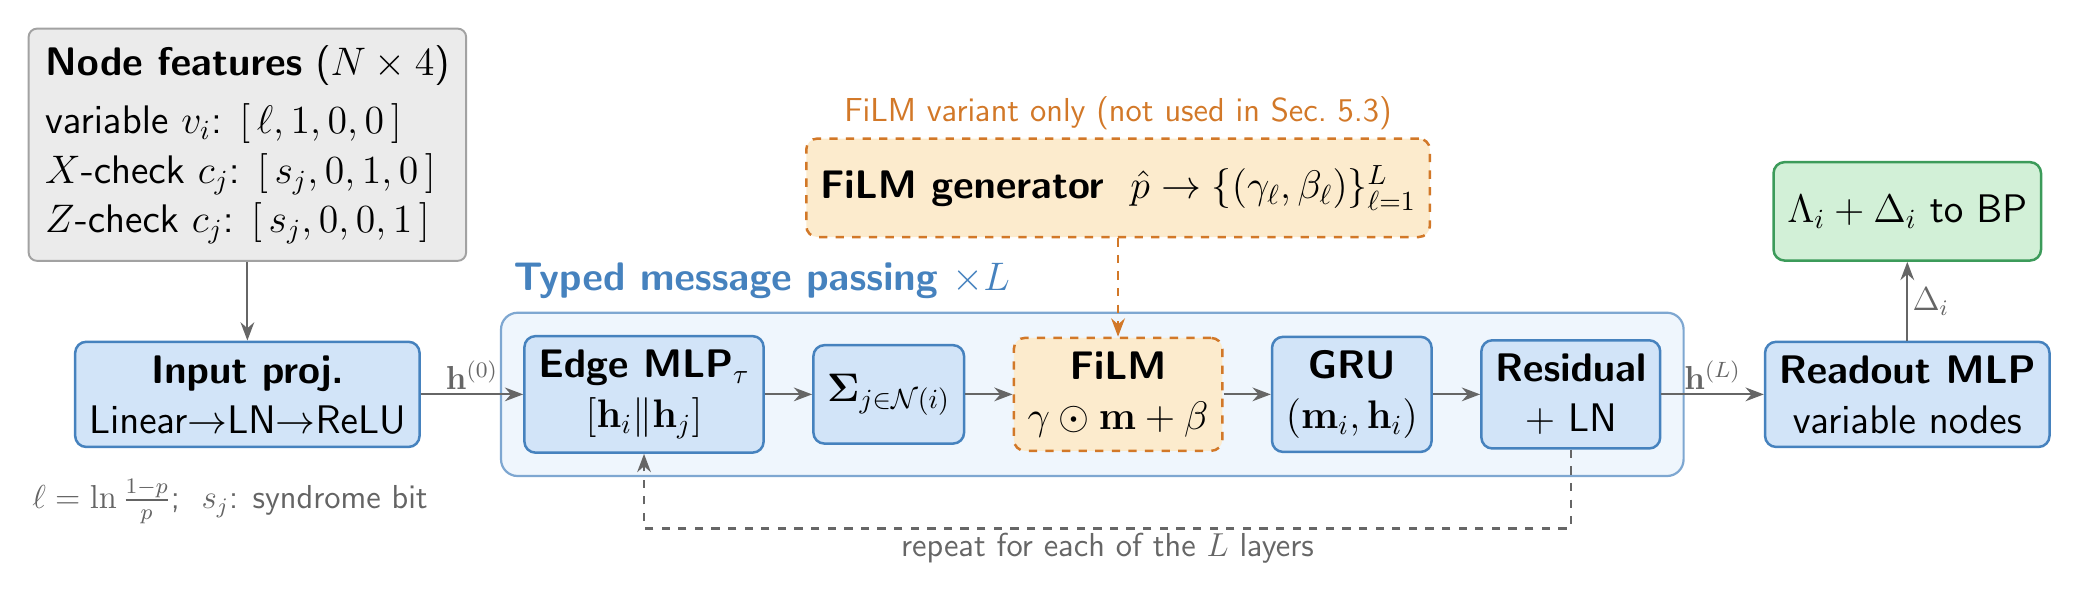
\begin{tikzpicture}[
    >=Stealth,
    font=\sffamily\Large,
    io/.style   = {rectangle, draw=iogray!60, fill=iofill, line width=0.7pt,
                   rounded corners=3pt, align=left, inner sep=6pt},
    gnn/.style  = {rectangle, draw=gnnblue, fill=gnnfill, line width=0.9pt,
                   rounded corners=4pt, align=center, minimum height=1.25cm, inner sep=5pt},
    film/.style = {rectangle, draw=filmorange, fill=fillfill, line width=0.9pt,
                   rounded corners=4pt, align=center, dashed, minimum height=1.25cm, inner sep=5pt},
    bp/.style   = {rectangle, draw=bpgreen, fill=bpfill, line width=0.9pt,
                   rounded corners=4pt, align=center, minimum height=1.25cm, inner sep=5pt},
    arr/.style  = {->, thick, black!60},
    lbl/.style  = {font=\sffamily\large, inner sep=1.5pt},
]

% ---- input features (left column) -----------------------------------------
\node[io] (feat) at (0,0) {%
  \textbf{Node features} ($N\times 4$)\\[3pt]
  variable $v_i$: $[\,\ell,1,0,0\,]$\\
  $X$-check $c_j$: $[\,s_j,0,1,0\,]$\\
  $Z$-check $c_j$: $[\,s_j,0,0,1\,]$};
\node[gnn, below=1.0cm of feat] (proj) {\textbf{Input proj.}\\Linear$\to$LN$\to$ReLU};
\draw[arr] (feat.south) -- (proj.north);

% ---- message-passing layer -------------------------------------------------
\node[gnn, right=1.3cm of proj] (msg) {\textbf{Edge MLP}$_{\tau}$\\$[\mathbf{h}_i\|\mathbf{h}_j]$};
\node[gnn, right=0.6cm of msg] (agg) {$\boldsymbol{\Sigma}_{j\in\mathcal{N}(i)}$};
\node[film, right=0.6cm of agg] (filmop) {\textbf{FiLM}\\$\gamma\odot\mathbf{m}+\beta$};
\node[gnn, right=0.6cm of filmop] (gru) {\textbf{GRU}\\$(\mathbf{m}_i,\mathbf{h}_i)$};
\node[gnn, right=0.6cm of gru] (res) {\textbf{Residual}\\+ LN};
\begin{scope}[on background layer]
  \node[draw=gnnblue!70, fill=gnnfill!35, rounded corners=6pt, line width=0.8pt,
        inner xsep=8pt, inner ysep=8pt, fit=(msg)(agg)(filmop)(gru)(res)] (layer) {};
\end{scope}
\node[font=\sffamily\Large\bfseries, text=gnnblue, anchor=south west] at ($(layer.north west)+(0.05,0.05)$)
     {Typed message passing $\times L$};

\draw[arr] (proj.east) -- node[lbl, above] {$\mathbf{h}^{(0)}$} (msg.west);
\draw[arr] (msg) -- (agg);
\draw[arr] (agg) -- (filmop);
\draw[arr] (filmop) -- (gru);
\draw[arr] (gru) -- (res);
\draw[arr, dashed] (res.south) -- ++(0,-1.0) -| node[lbl, pos=0.25, below] {repeat for each of the $L$ layers} (msg.south);

% ---- readout (right column) -------------------------------------------------
\node[gnn, right=1.3cm of res] (read) {\textbf{Readout MLP}\\variable nodes};
\node[bp, above=1.0cm of read] (out) {$\Lambda_i+\Delta_i$ to BP};
\draw[arr] (res.east) -- node[lbl, above] {$\mathbf{h}^{(L)}$} (read.west);
\draw[arr] (read.north) -- node[lbl, right] {$\Delta_i$} (out.south);

% ---- FiLM generator (FiLM variant only) -----------------------------------------
\node[film, above=1.25cm of filmop] (filmgen) {\textbf{FiLM generator}\ \ $\hat{p}\to\{(\gamma_\ell,\beta_\ell)\}_{\ell=1}^{L}$};
\node[lbl, above=1pt of filmgen, text=filmorange] {FiLM variant only (not used in Sec.~5.3)};
\draw[arr, filmorange, dashed] (filmgen.south) -- (filmop.north);

\node[lbl, iogray, below=3pt of feat.south west, anchor=north west, xshift=0pt, yshift=-2.6cm] {$\ell=\ln\frac{1-p}{p}$; \ $s_j$: syndrome bit};
\end{tikzpicture}
\end{document}
